\section{Rakefile開発に関するメモ}
\subsection{日本語のcode listings}
日本語のjlistingの使用法が判明しました.
listingsでは日本語表示がちゃんとなされません.そこで,
\begin{quote}\begin{verbatim}
\usepackage{listings,jlisting}
\end{verbatim}\end{quote}
とします.これで,日本語が含まれたcodeも綺麗に表示してくれます.

\subsection{文献参照のシステム}
latexへ文献参照を渡すために,下記のようなフォーマットでの記述を行う.
\begin{lstlisting}[style=customCsh,basicstyle={\scriptsize\ttfamily}]
図{{ref(fig:SystemOverview)}}に卒論編集システムの概観を示しています.

!!!caption: (fig:SystemOverview)卒論編集システムの概観.
{{attach_view(hikiutils_bob.006.jpeg)}}

*基本的な使い方{{cite(listings1)}}
*独自のカラー化{{cite(listings2)}}
!reference:
:listings1:[[http://d.hatena.ne.jp/mallowlabs/20061226/1167137637]]
:listings2:[[http://www.ipc.akita-nct.ac.jp/~yamamoto/comp/latex/make_doc/source/source.html]]
\end{lstlisting}
これをlatexにかけると次の通りになります.(体裁は乱れている)

図\ref{fig:SystemOverview}に卒論編集システムの概観を示しています.

\begin{figure}[htbp]\begin{center}
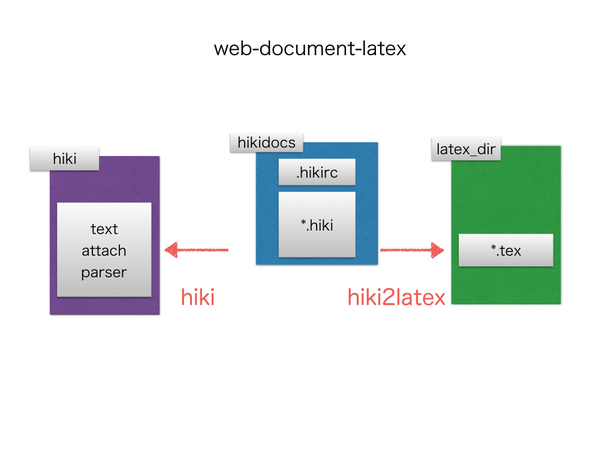
\includegraphics[width=10cm,bb= 0 0 737 453]{../figs/./hikiutils_bob.006.jpeg}
\caption{卒論編集システムの概観.}
\label{fig:SystemOverview}
\label{default}\end{center}\end{figure}
\begin{itemize}
\item 基本的な使い方\cite{listings1}
\item 独自のカラー化\cite{listings2}
\end{itemize}
\begin{thebibliography}{99}
\bibitem{listings1}  \verb|http://d.hatena.ne.jp/mallowlabs/20061226/1167137637|
\bibitem{listings2}  \verb|http://www.ipc.akita-nct.ac.jp/~yamamoto/comp/latex/make_doc/source/source.html|
\end{thebibliography}
\subsection{システムの概要}
卒論編集システム開発時のメモです.図\ref{fig:SystemOverview}に卒論編集システムの概観を示しています.

hikiシステムとの同期は,hikiutilsのhikiが下請けしている.
一方,latex\_dirへの出力はlatex2hikiが引き受けている.
フォーマットをいじるときには,基本的に
\begin{description}
\item[hikiへ] hikiがやるので,そのまえにtmp.txtへ写して置換

\item[texへ] latex2hikiからの出力(tmp.txt)を処理してtexへ

\end{description}
で行っている,あるいはおこなう.

\subsection{rake mk\_toc}
latexが作成するtableofcontentsの実態であるtocファイルからhiki用のtoc.hikiを作成する.

